\documentclass{beamer}
\usepackage{amsmath}
\usepackage[english]{babel} %set language; note: after changing this, you need to delete all auxiliary files to recompile
\usepackage[utf8]{inputenc} %define file encoding; latin1 is the other often used option
\usepackage{csquotes} % provides context sensitive quotation facilities
\usepackage{graphicx} %allows for inserting figures
\usepackage{booktabs} % for table formatting without vertical lines
\usepackage{textcomp} % allow for example using the Euro sign with \texteuro
\usepackage{stackengine}
\usepackage{wasysym}
\usepackage{tikzsymbols}
\usepackage{textcomp}
\usepackage{xcolor}
\usepackage[dvipsnames]{xcolor}
\usepackage{colortbl}
\usepackage{adjustbox}
\newcommand{\bubblethis}[2]{
        \tikz[remember picture,baseline]{\node[anchor=base,inner sep=0,outer sep=0]%
        (#1) {\underline{#1}};\node[overlay,cloud callout,callout relative pointer={(0.2cm,-0.7cm)},%
        aspect=2.5,fill=yellow!90] at ($(#1.north)+(-0.5cm,1.6cm)$) {#2};}%
    }%
\tikzset{face/.style={shape=circle,minimum size=4ex,shading=radial,outer sep=0pt,
        inner color=white!50!yellow,outer color= yellow!70!orange}}
%% Some commands to make the code easier
\newcommand{\emoticon}[1][]{%
  \node[face,#1] (emoticon) {};
  %% The eyes are fixed.
  \draw[fill=white] (-1ex,0ex) ..controls (-0.5ex,0.2ex)and(0.5ex,0.2ex)..
        (1ex,0.0ex) ..controls ( 1.5ex,1.5ex)and( 0.2ex,1.7ex)..
        (0ex,0.4ex) ..controls (-0.2ex,1.7ex)and(-1.5ex,1.5ex)..
        (-1ex,0ex)--cycle;}
\newcommand{\pupils}{
  %% standard pupils
  \fill[shift={(0.5ex,0.5ex)},rotate=80] 
       (0,0) ellipse (0.3ex and 0.15ex);
  \fill[shift={(-0.5ex,0.5ex)},rotate=100] 
       (0,0) ellipse (0.3ex and 0.15ex);}

\newcommand{\emoticonname}[1]{
  \node[below=1ex of emoticon,font=\footnotesize,
        minimum width=4cm]{#1};}
\usepackage{scalerel}
\usetikzlibrary{positioning}
\usepackage{xcolor,amssymb}
\newcommand\dangersignb[1][2ex]{%
  \scaleto{\stackengine{0.3pt}{\scalebox{1.1}[.9]{%
  \color{red}$\blacktriangle$}}{\tiny\bfseries !}{O}{c}{F}{F}{L}}{#1}%
}
\newcommand\dangersignw[1][2ex]{%
  \scaleto{\stackengine{0.3pt}{\scalebox{1.1}[.9]{%
  \color{red}$\blacktriangle$}}{\color{white}\tiny\bfseries !}{O}{c}{F}{F}{L}}{#1}%
}
\usepackage{fontawesome} % Social Icons
\usepackage{epstopdf} % allow embedding eps-figures
\usepackage{tikz} % allows drawing figures
\usepackage{amsmath,amssymb,amsthm} %advanced math facilities
\usepackage{lmodern} %uses font that support italic and bold at the same time
\usepackage{hyperref}
\usepackage{tikz}
\hypersetup{
    colorlinks=true,
    linkcolor=blue,
    filecolor=magenta,      
    urlcolor=blue,
}
\usepackage{tcolorbox}
%add citation management using BibLaTeX
\usepackage[citestyle=authoryear-comp, %define style for citations
    bibstyle=authoryear-comp, %define style for bibliography
    maxbibnames=10, %maximum number of authors displayed in bibliography
    minbibnames=1, %minimum number of authors displayed in bibliography
    maxcitenames=3, %maximum number of authors displayed in citations before using et al.
    minnames=1, %maximum number of authors displayed in citations before using et al.
    datezeros=false, % do not print dates with leading zeros
    date=long, %use long formats for dates
    isbn=false,% show no ISBNs in bibliography (applies only if not a mandatory field)
    url=false,% show no urls in bibliography (applies only if not a mandatory field)
    doi=false, % show no dois in bibliography (applies only if not a mandatory field)
    eprint=false, %show no eprint-field in bibliography (applies only if not a mandatory field)
    backend=biber %use biber as the backend; backend=bibtex is less powerful, but easier to install
    ]{biblatex}
\addbibresource{../mybibfile.bib} %define bib-file located one folder higher


\usefonttheme[onlymath]{serif} %set math font to serif ones

\definecolor{beamerblue}{rgb}{0.2,0.2,0.7} %define beamerblue color for later use

%%% defines highlight command to set text blue
\newcommand{\highlight}[1]{{\color{blue}{#1}}}


%%%%%%% commands defining backup slides so that frame numbering is correct

\newcommand{\backupbegin}{
   \newcounter{framenumberappendix}
   \setcounter{framenumberappendix}{\value{framenumber}}
}
\newcommand{\backupend}{
   \addtocounter{framenumberappendix}{-\value{framenumber}}
   \addtocounter{framenumber}{\value{framenumberappendix}}
}

%%%% end of defining backup slides

%Specify figure caption, see also http://tex.stackexchange.com/questions/155738/caption-package-not-working-with-beamer
\setbeamertemplate{caption}{\insertcaption} %redefines caption to remove label "Figure".
%\setbeamerfont{caption}{size=\scriptsize,shape=\itshape,series=\bfseries} %sets figure  caption bold and italic and makes it smaller


\usetheme{Boadilla}

%set options of hyperref package
\hypersetup{
    bookmarksnumbered=true, %put section numbers in bookmarks
    naturalnames=true, %use LATEX-computed names for links
    citebordercolor={1 1 1}, %color of border around cites, here: white, i.e. invisible
    linkbordercolor={1 1 1}, %color of border around links, here: white, i.e. invisible
    colorlinks=true, %color links
    anchorcolor=black, %set color of anchors
    linkcolor=beamerblue, %set link color to beamer blue
    citecolor=blue, %set cite color to beamer blue
    pdfpagemode=UseThumbs, %set default mode of PDF display
    breaklinks=true, %break long links
    pdfstartpage=1 %start at first page
    }


\newtcolorbox{boxA}{
    fontupper = \bf,
    boxrule = 1.5pt,
    colframe = black % frame color
}
\newtcolorbox{boxB}{
    boxrule = 1.5pt,
    colframe = blue!70!black,, % frame color
    colback = blue!7!white,
}

% --------------------
% Overall information
% --------------------
\title[Economía I]{Economía I \vspace{3mm}
\\ Magistral 20 \vspace{3mm} \\ Teoría del Crecimiento}
\date{}
\author[Victoria Rosino]{Victoria Rosino}
\vspace{0.3cm}
\institute[]{Universidad de San Andrés} 

\begin{document}

\begin{frame}
\vspace{0.3cm}
\titlepage
\centering
\vspace{-0.9cm}

\includegraphics[scale=0.3]{Slides Principios de Economia/Figures/udesa_logo.jpg} 
\end{frame}


\begin{frame}
\frametitle{Tomemos una economía}

\begin{figure}[H]
\begin{center}
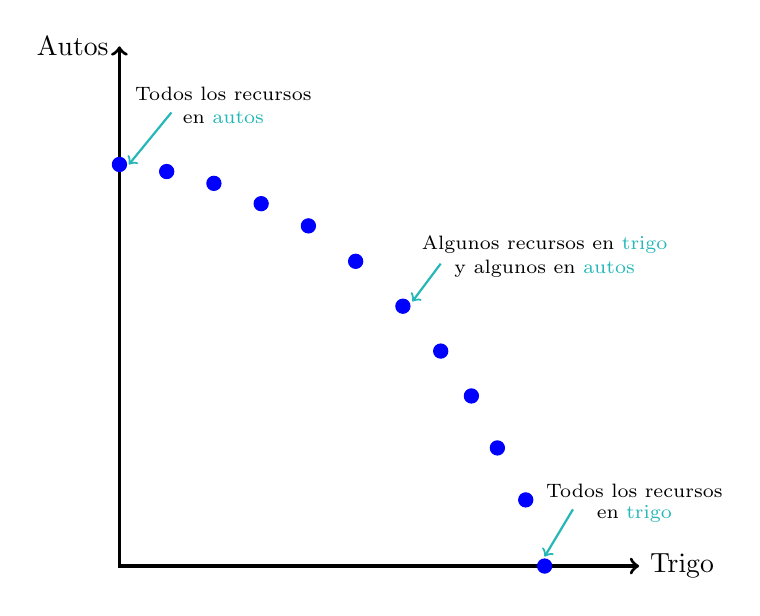
\begin{tikzpicture}[scale=0.6]

\draw[very thick,<->] (0,11) node[left]{Autos}--(0,0)--(11,0) node[right]{Trigo};

\draw[fill, blue] (0,8.5) circle [radius =0.15] ;
\draw[fill, blue] (1,8.35) circle [radius =0.15] ;
\draw[fill, blue] (2,8.1) circle [radius =0.15];
\draw[fill, blue] (3,7.67) circle [radius =0.15] ;
\draw[fill, blue] (4,7.2) circle [radius =0.15] ;
\draw[fill, blue] (5,6.45) circle [radius =0.15] ;
\draw[fill, blue] (6,5.5) circle [radius =0.15] ; 
\draw[fill, blue] (6.8,4.55) circle [radius =0.15] ;
\draw[fill, blue] (7.45,3.6) circle [radius =0.15] ;
\draw[fill, blue] (8,2.5) circle [radius =0.15] ;
\draw[fill, blue] (8.6,1.4) circle [radius =0.15] ;
\draw[fill, blue] (9,0) circle [radius =0.15] ;

\draw[fill, BlueGreen, ->, thick] (1.1,9.6) --(0.2,8.5) ;
\node[] at (2.2,10) {\scriptsize Todos los recursos};
\node[] at (2.2,9.5) {\scriptsize en \textcolor{BlueGreen}{autos}};

\draw[fill, BlueGreen, ->, thick] (6.8,6.4) --(6.2,5.6) ;
\node[] at (9,6.8) {\scriptsize Algunos recursos en \textcolor{BlueGreen}{trigo}};
\node[] at (9,6.3) {\scriptsize y algunos en \textcolor{BlueGreen}{autos}};


\draw[fill, BlueGreen, ->, thick] (9.6,1.2) --(9,0.2) ;
\node[] at (10.9,1.6) {\scriptsize Todos los recursos};
\node[] at (10.9,1.1) {\scriptsize en \textcolor{BlueGreen}{trigo}};

\end{tikzpicture}
\end{center}
\end{figure}

\end{frame}


\begin{frame}
\frametitle{Frontera de posibilidades de producción}

\begin{figure}[H]
\renewcommand{\figurename}{Figure}
\begin{center}
\begin{tikzpicture}[scale=0.6]

\draw[very thick,<->] (0,11) node[left]{Autos}--(0,0)--(11,0) node[right]{Trigo};

\draw[fill, blue] (0,8.5) circle [radius =0.15] ;
\draw[fill, blue] (1,8.35) circle [radius =0.15] ;
\draw[fill, blue] (2,8.1) circle [radius =0.15];
\draw[fill, blue] (3,7.67) circle [radius =0.15] ;
\draw[fill, blue] (4,7.2) circle [radius =0.15] ;
\draw[fill, blue] (5,6.45) circle [radius =0.15] ;
\draw[fill, blue] (6,5.5) circle [radius =0.15] ;
\draw[fill, blue] (6.8,4.55) circle [radius =0.15];
\draw[fill, blue] (7.45,3.6) circle [radius =0.15];
\draw[fill, blue] (8,2.5) circle [radius =0.15];
\draw[fill, blue] (8.6,1.4) circle [radius =0.15] ;
\draw[fill, blue] (9,0) circle [radius =0.15] ;

\draw[thin] (0,8.5).. controls (6,8.25) and (9, 1) .. (9,0);
\end{tikzpicture}
\end{center}

\end{figure}
\end{frame}

\begin{frame}
\frametitle{Frontera de posibilidades de producción}

\begin{figure}[H]
\begin{center}
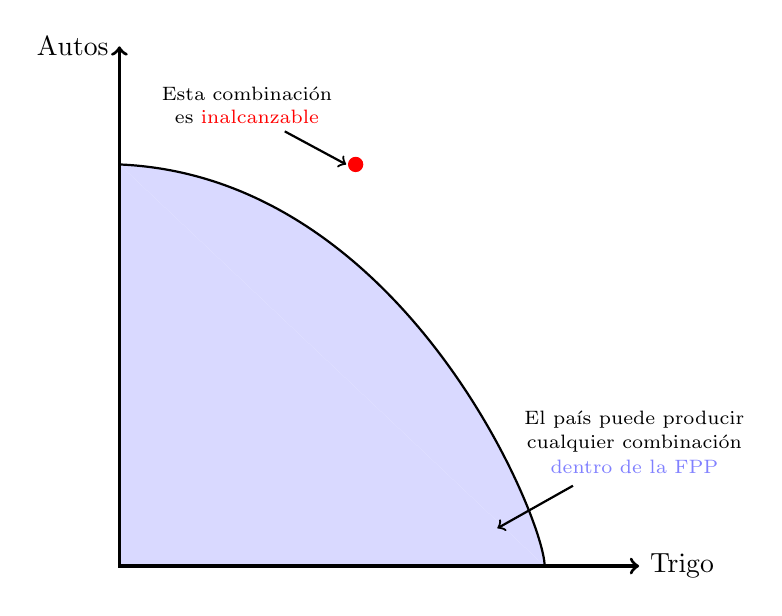
\begin{tikzpicture}[scale=0.6]

\draw[fill,blue!15] (0,8.5).. controls (6,8.25) and (9, 1) .. (9,0) ;
\draw[fill,blue!15] (0,8.5) -- (0,0) -- (9,0) ;
\draw[very thick,<->] (0,11) node[left]{Autos}--(0,0)--(11,0) node[right]{Trigo};
\draw[fill, red] (5,8.5) circle [radius =0.15] ;
\draw[thin, thick] (0,8.5).. controls (6,8.25) and (9, 1) .. (9,0);
\draw[fill, ->, thick] (3.5,9.2) --(4.8,8.5) ;
\node[] at (2.7,10) {\scriptsize Esta combinación};
\node[] at (2.7,9.5) {\scriptsize es \textcolor{red}{inalcanzable}};
\draw[fill, ->, thick] (9.6,1.7) --(8,0.8) ;
\node[] at (10.9,3.1) {\scriptsize El país puede producir};
\node[] at (10.9,2.6) {\scriptsize cualquier combinación};
\node[] at (10.9,2.1) {\scriptsize \textcolor{blue!50}{dentro de la FPP}};

\end{tikzpicture}
\end{center}
\end{figure}

\end{frame}

\begin{frame}
\frametitle{Misma frontera}

\begin{figure}[H]
\renewcommand{\figurename}{Figure}
\begin{center}
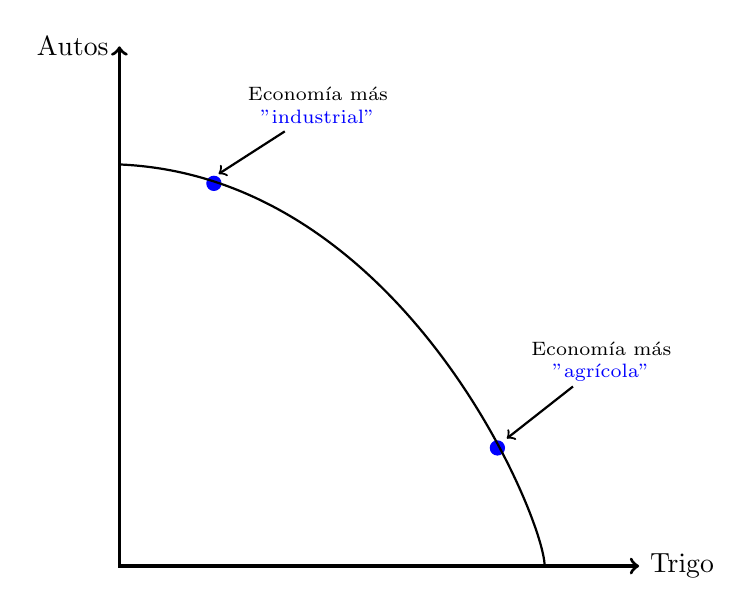
\begin{tikzpicture}[scale=0.6]

\draw[very thick,<->] (0,11) node[left]{Autos}--(0,0)--(11,0) node[right]{Trigo};

\draw[fill, blue] (2,8.1) circle [radius =0.15] ;
\draw[fill, blue] (8,2.5) circle [radius =0.15];
\draw[thin, thick] (0,8.5).. controls (6,8.25) and (9, 1) .. (9,0);

\draw[fill, ->, thick] (3.5,9.2) --(2.1,8.3) ;
\node[] at (4.2,10) {\scriptsize Economía más};
\node[] at (4.2,9.5) {\scriptsize \textcolor{blue}{"industrial"}};


\draw[fill, ->, thick] (9.6,3.8) --(8.2,2.7) ;
\node[] at (10.2,4.6) {\scriptsize  Economía más};
\node[] at (10.2,4.1) {\scriptsize \textcolor{blue}{"agrícola"}};

\end{tikzpicture}
\end{center}

\end{figure}
\end{frame}


\begin{frame}
\frametitle{Mejora en la tecnología de cultivo}

\begin{figure}[H]
\renewcommand{\figurename}{Figure}
\begin{center}
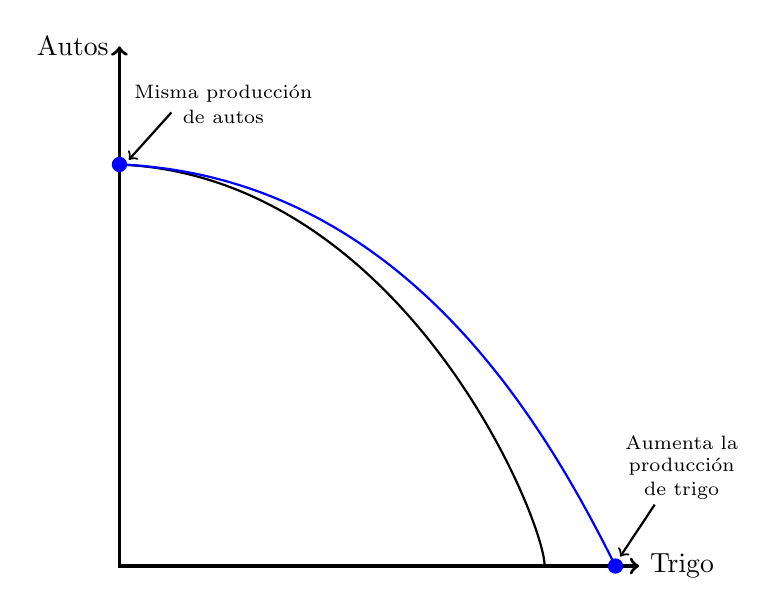
\begin{tikzpicture}[scale=0.6]

\draw[very thick,<->] (0,11) node[left]{Autos}--(0,0)--(11,0) node[right]{Trigo};

\draw[thin, thick] (0,8.5).. controls (6,8.25) and (9, 1) .. (9,0);
\draw[thin, thick, blue] (0,8.5).. controls (6,8.25) and (9, 3) .. (10.5,0);

\draw[fill, blue] (0,8.5) circle [radius =0.15] ;
\draw[fill, ->, thick] (1.1,9.6) --(0.2,8.6) ;
\node[] at (2.2,10) {\scriptsize Misma producción};
\node[] at (2.2,9.5) {\scriptsize de autos};

\draw[fill, blue] (10.5,0) circle [radius =0.15] ;
\draw[fill, ->, thick] (11.33,1.3) --(10.6,0.2) ;
\node[] at (11.9,2.6) {\scriptsize Aumenta la};
\node[] at (11.9,2.1) {\scriptsize producción};
\node[] at (11.9,1.6) {\scriptsize de trigo};

\end{tikzpicture}
\end{center}

\end{figure}
\end{frame}

\begin{frame}
\frametitle{Cambio en los factores}

\begin{figure}[H]
\begin{center}
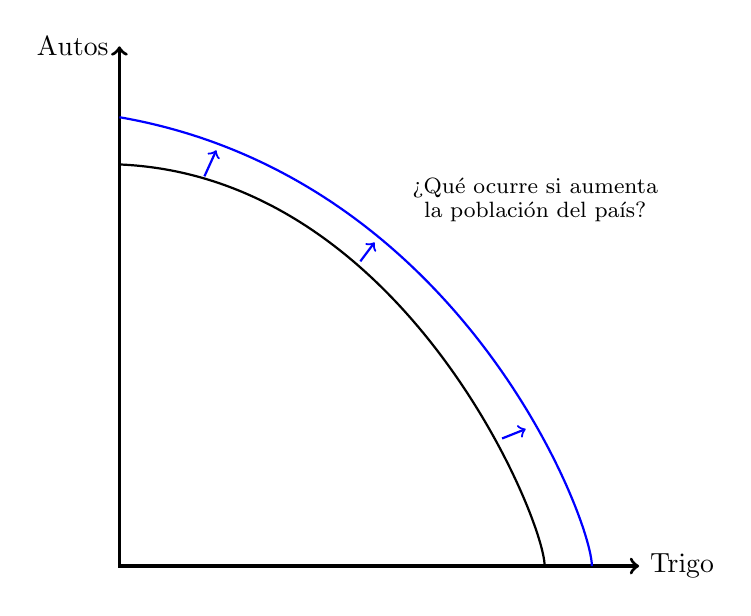
\begin{tikzpicture}[scale=0.6]

\draw[very thick,<->] (0,11) node[left]{Autos}--(0,0)--(11,0) node[right]{Trigo};

\draw[thin, thick] (0,8.5).. controls (6,8.25) and (9, 1) .. (9,0);
\draw[thin, thick, blue] (0,9.5).. controls (7.2,8.25) and (10, 1) .. (10,0);

\draw[fill, ->,blue, thick] (5.1,6.45) --(5.4,6.85) ;
\draw[fill, ->,blue, thick] (8.1,2.7) --(8.6,2.9) ;
\draw[fill, ->,blue, thick] (1.8,8.25) -- (2.05,8.8) ;
\node[] at (8.8,8) {\footnotesize ¿Qué ocurre si aumenta};
\node[] at (8.8,7.5) {\footnotesize la población del país?};
\end{tikzpicture}
\end{center}
\end{figure}

\end{frame}

\begin{frame}
\frametitle{Shock exógeno}
\begin{figure}[H]
\begin{center}
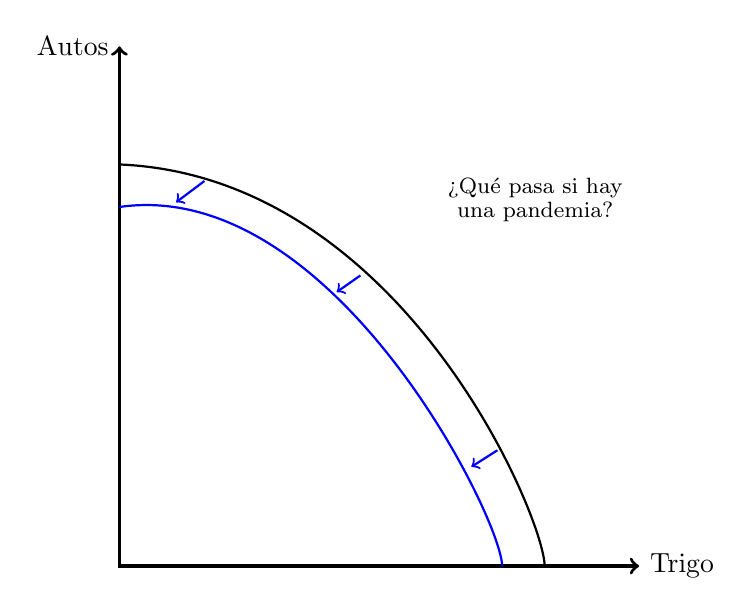
\begin{tikzpicture}[scale=0.6]

\draw[very thick,<->] (0,11) node[left]{Autos}--(0,0)--(11,0) node[right]{Trigo};

\draw[thin, thick] (0,8.5).. controls (6,8.25) and (9, 1) .. (9,0);
\draw[thin, thick, blue] (0,7.6).. controls (4.5,8.25) and (8.1,1) .. (8.1,0);

\draw[fill, ->,blue, thick] (5.1,6.15) --(4.6,5.8) ;
\draw[fill, ->,blue, thick] (8,2.45) --(7.45,2.1) ;
\draw[fill, ->,blue, thick] (1.8,8.15) -- (1.2,7.7) ;
\node[] at (8.8,8) {\footnotesize ¿Qué pasa si hay};
\node[] at (8.8,7.5) {\footnotesize una pandemia?};
\end{tikzpicture}
\end{center}
\end{figure}
\end{frame}

\begin{frame}
\frametitle{Cambios en el equilibrio}

\begin{figure}[H]
\begin{center}
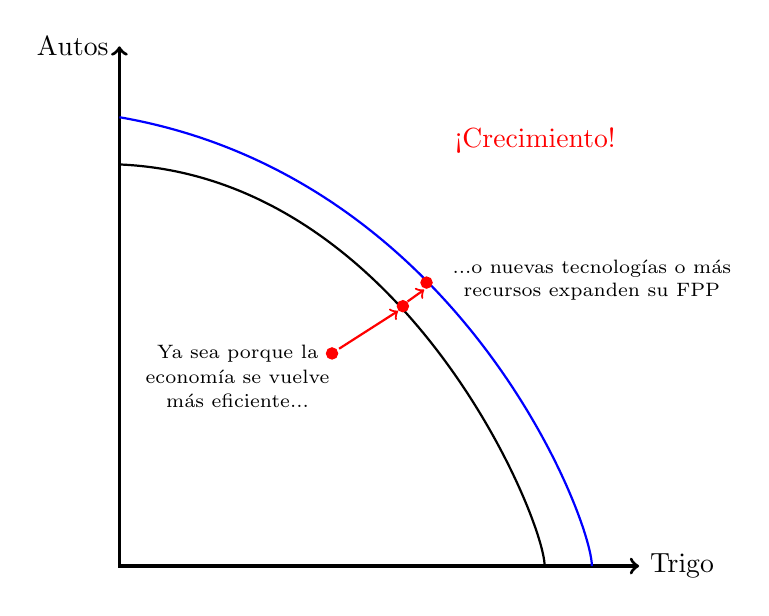
\begin{tikzpicture}[scale=0.6]

\draw[very thick,<->] (0,11) node[left]{Autos}--(0,0)--(11,0) node[right]{Trigo};

\draw[thin, thick] (0,8.5).. controls (6,8.25) and (9, 1) .. (9,0);
\draw[thin, thick, blue] (0,9.5).. controls (7.2,8.25) and (10, 1) .. (10,0);


\node[red] at (8.8,9) {¡Crecimiento!};

\draw[fill, red] (4.5,4.5) circle [radius =0.12] ;
\draw[fill, ->,red, thick] (4.65,4.6) -- (5.9,5.4) ;
\draw[fill, ->,red, thick] (6.1,5.6) -- (6.45,5.85) ;
\draw[fill, red] (6,5.5) circle [radius =0.12];
\draw[fill, red] (6.5,6) circle [radius =0.12];

\node[] at (2.5,4.5) {\scriptsize Ya sea porque la };
\node[] at (2.5,4) {\scriptsize economía se vuelve};
\node[] at (2.5,3.5) {\scriptsize más eficiente...};

\node[] at (10,6.3) {\scriptsize ...o nuevas tecnologías o más};
\node[] at (10,5.8) {\scriptsize recursos expanden su FPP};
\end{tikzpicture}
\end{center}
\end{figure}

\end{frame}

\begin{frame}
\frametitle{Luces nocturnas}
\begin{center}
    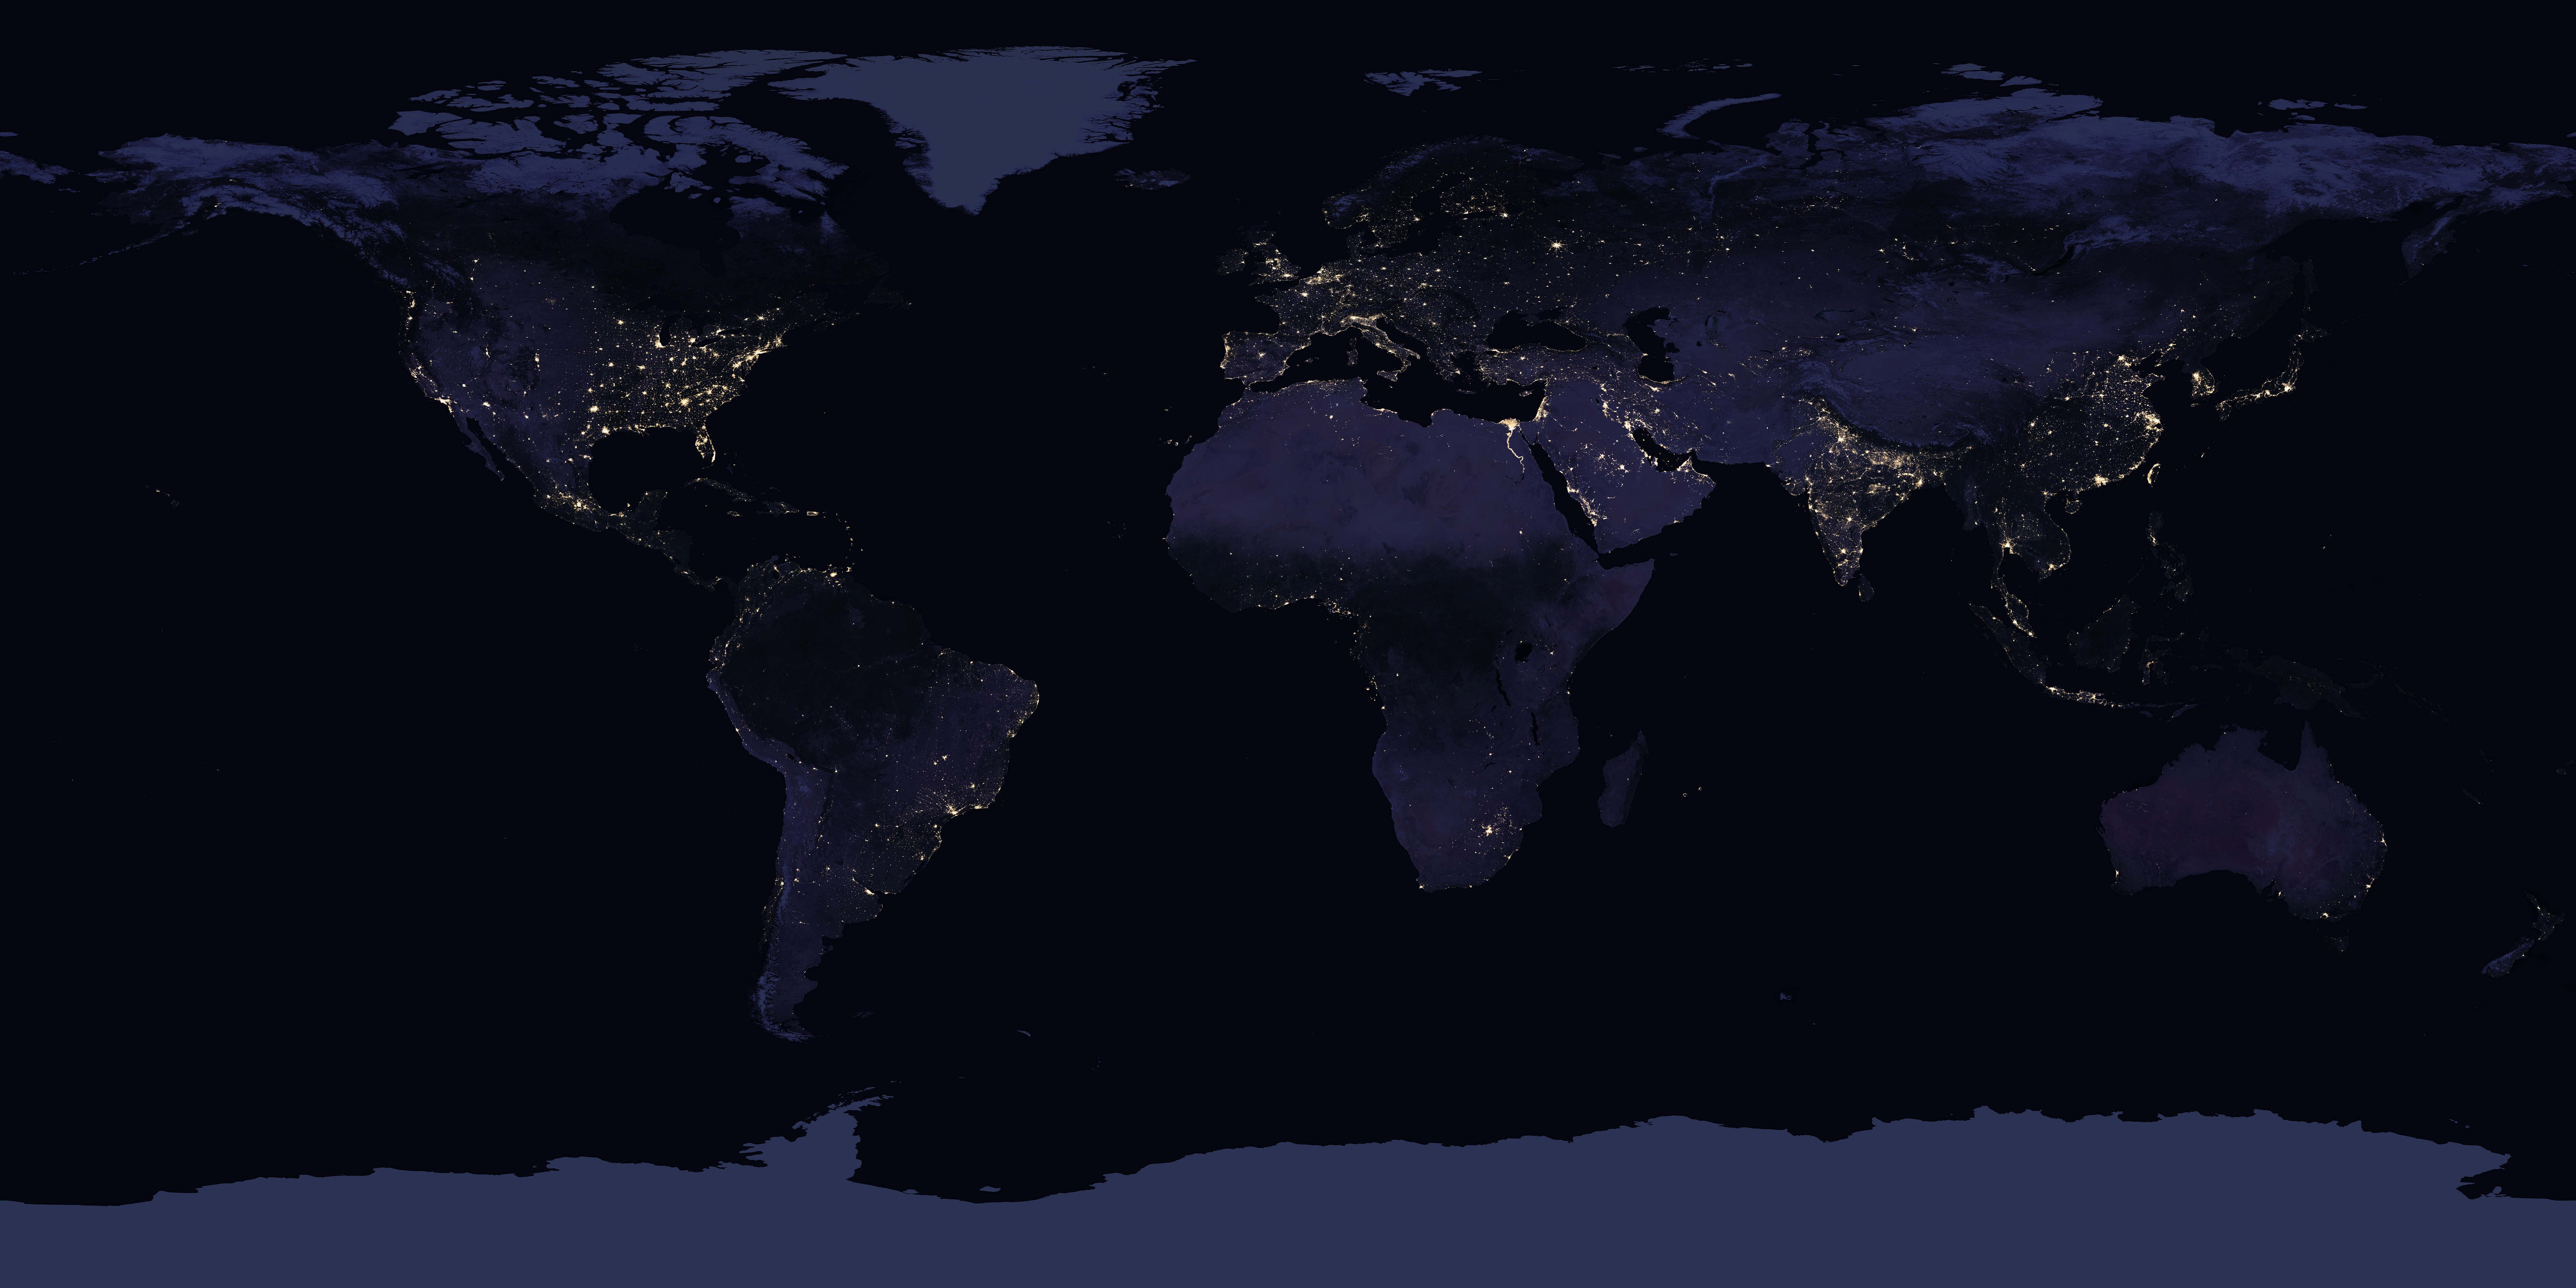
\includegraphics[scale=0.06]{Slides Principios de Economia/Tema_11.11_crecimiento2.jpg}
\end{center}
Fuente: \href{https://www.nasa.gov/feature/goddard/2017/new-night-lights-maps-open-up-possible-real-time-applications}{NASA}
\end{frame}

\begin{frame}
\frametitle{Crecimiento}
\begin{center}
    \href{https://ourworldindata.org/grapher/gdp-per-capita-worldbank} {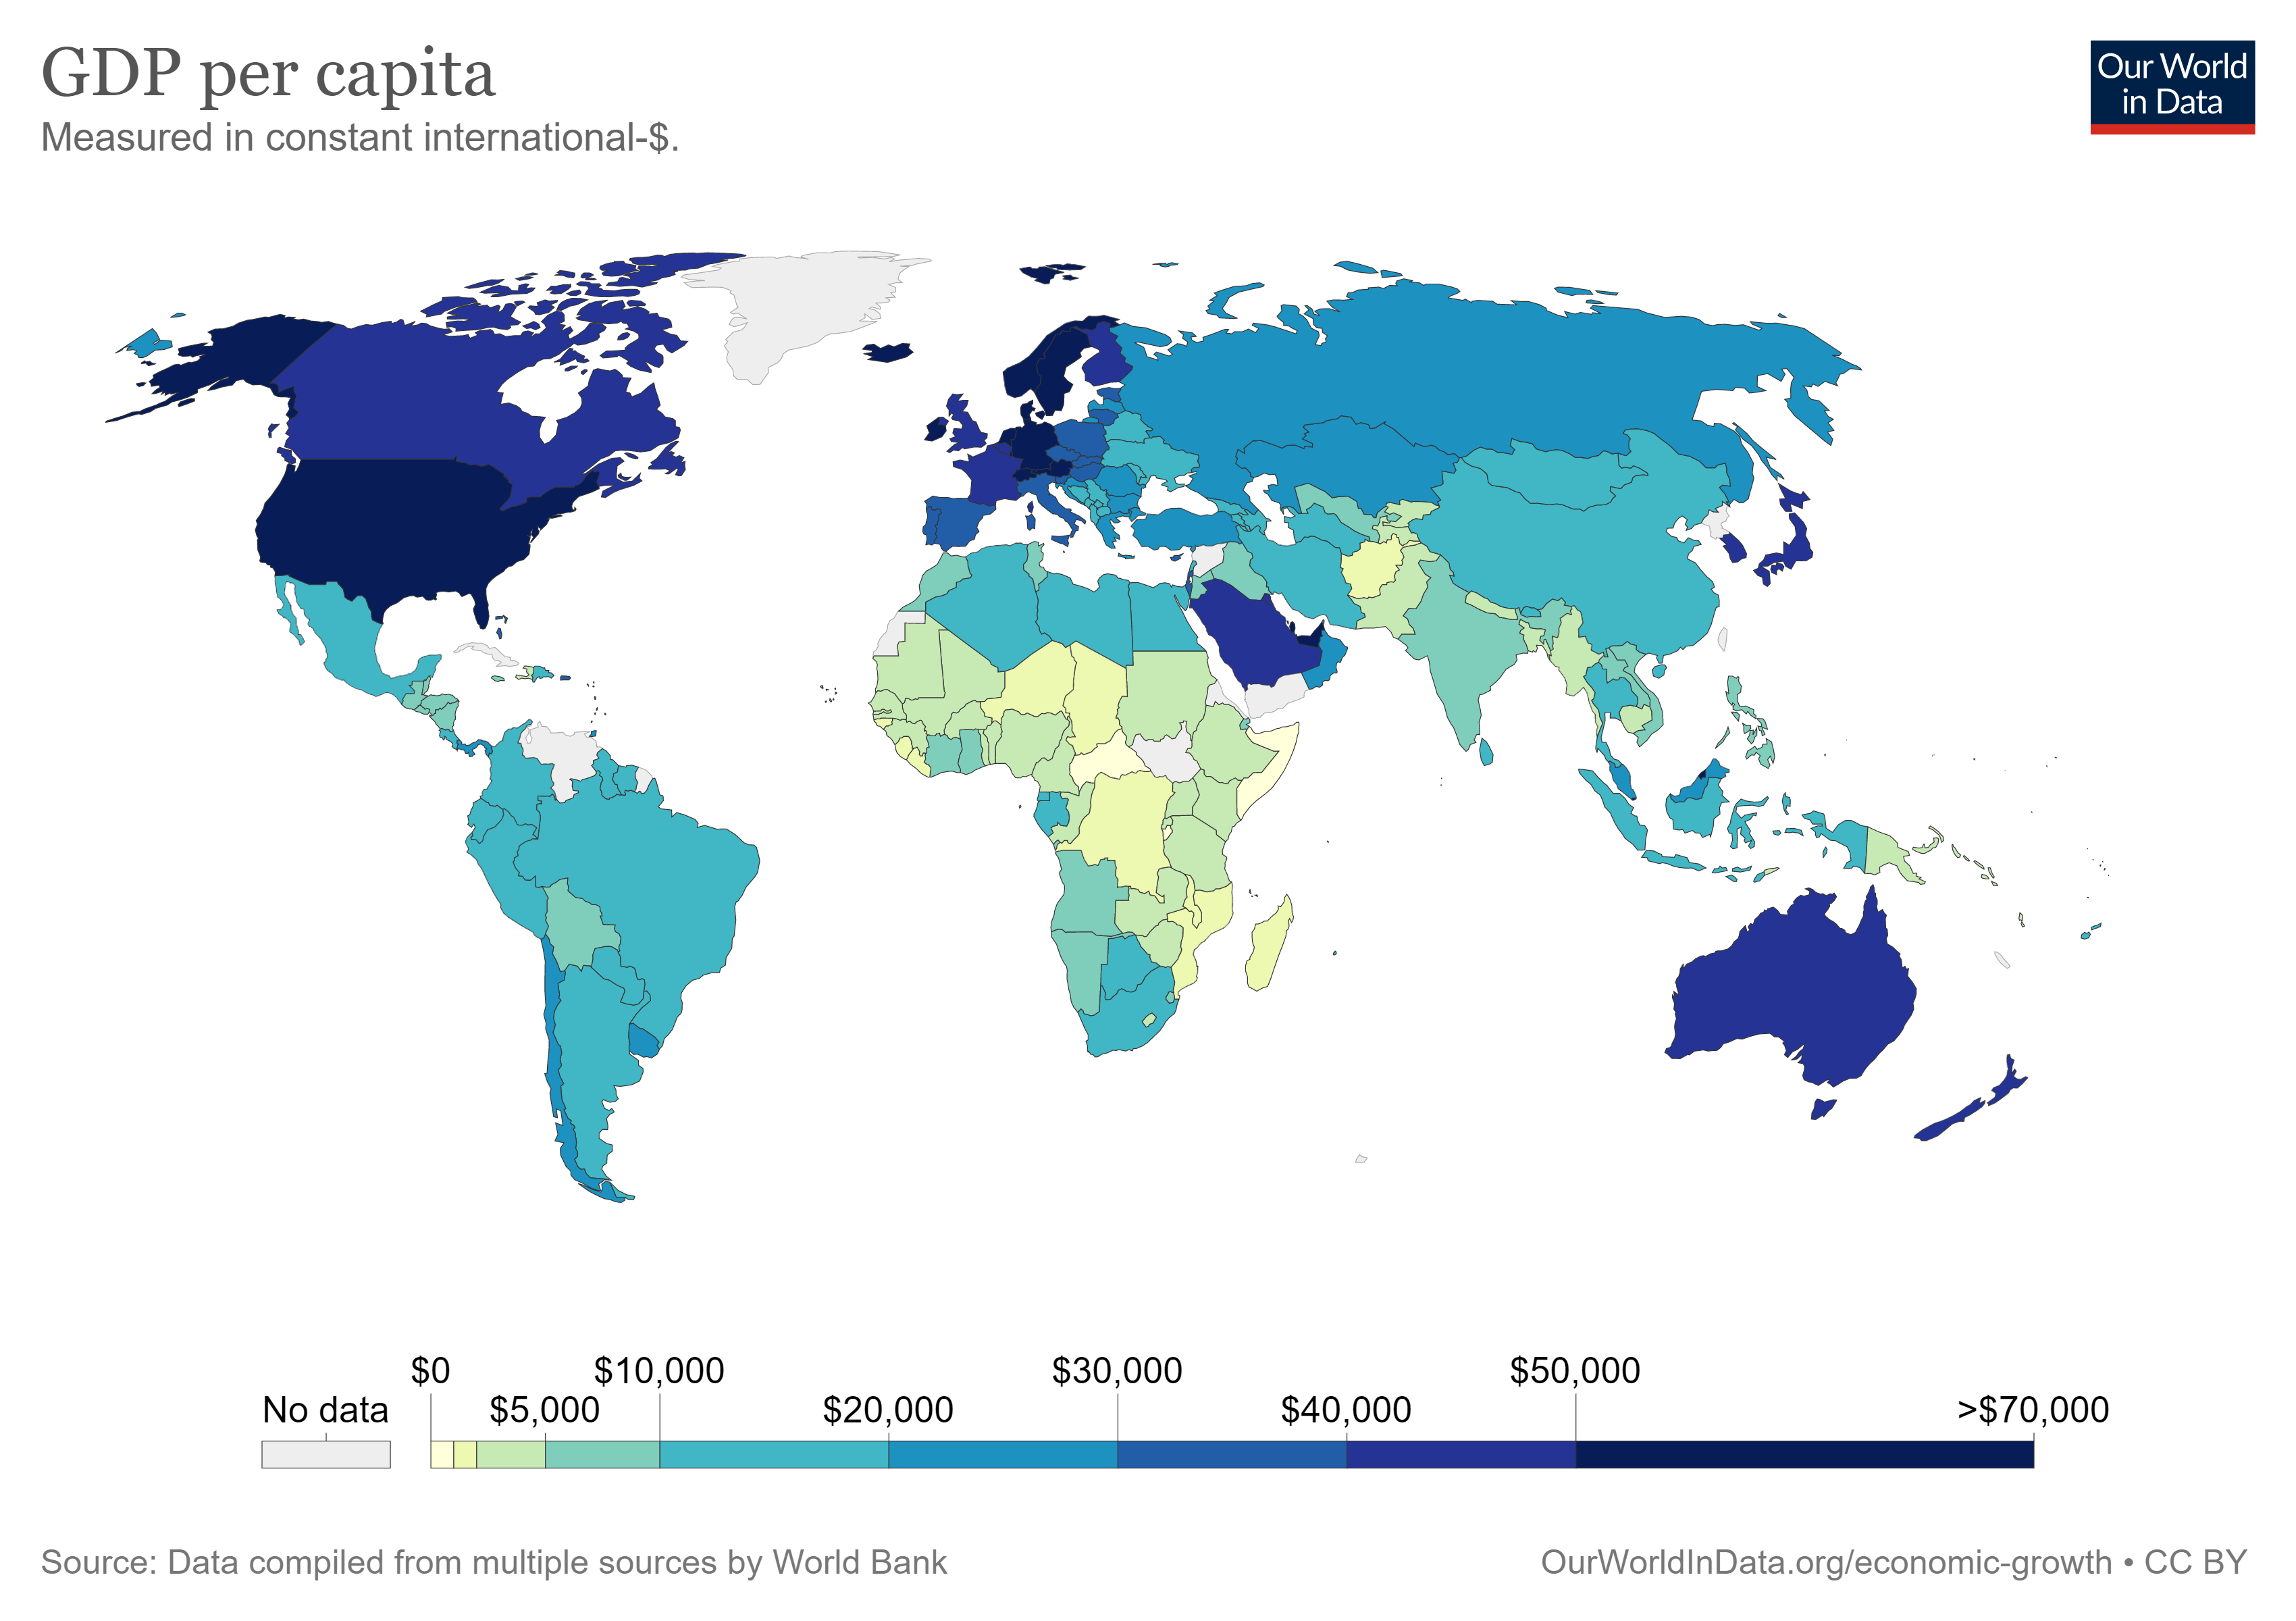
\includegraphics[width=0.9\textwidth]{Slides Principios de Economia/Figures/gdppc2020.png}}
\end{center}
\small Fuente: Our World in Data
\end{frame}

\begin{frame}{Crecimiento del GDP per cápita}
    \begin{figure} [H]   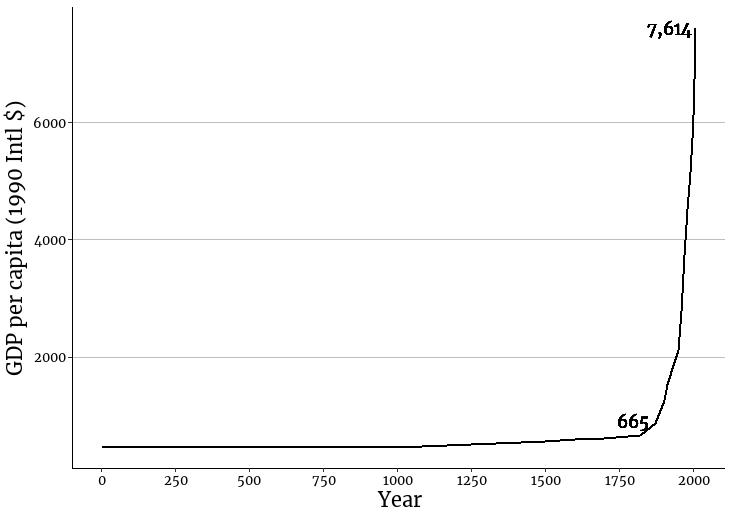
\includegraphics[scale=0.5]{Slides Principios de Economia/Figures/C17.1.png}
\end{figure}
\end{frame}

\begin{frame}{¿Qué generó el crecimiento explosivo?}
    \begin{itemize}
    \item \textbf{Revolución industrial (desde mediados del Siglo XVIII)}
    \begin{itemize}
        \item La máquina a vapor generó una potencialidad de expansión en la producción junto con los ferrocarriles y la industria textil produjeron un aumento en el nivel de vida sin precedentes.
    \end{itemize}

    \item \textbf{Constitución de EEUU (1787)}
     \begin{itemize}
        \item Fuerte contraste con el poder absolutista de los monarcas europeos.
        \item Fuertes restricciones al Estado y lo que éste podía hacer.
        \item La emergencia de los gobiernos republicanos con división de poderes implicó un cambio radical en la calidad de la gestión de los recursos públicos.
        \end{itemize}
        
    \item \textbf{Revolución francesa (1789)}
    \begin{itemize}
        \item Permitió la movilidad social.
        \item Se pasó de una sociedad estamental a una sociedad libre: mayor libertad para elegir los trabajos y ocupaciones según sus preferencias y capacidades.
    \end{itemize}
\end{itemize}
\end{frame}

%\begin{frame}{Felicidad y nivel de ingreso}
%    \begin{figure} [H]   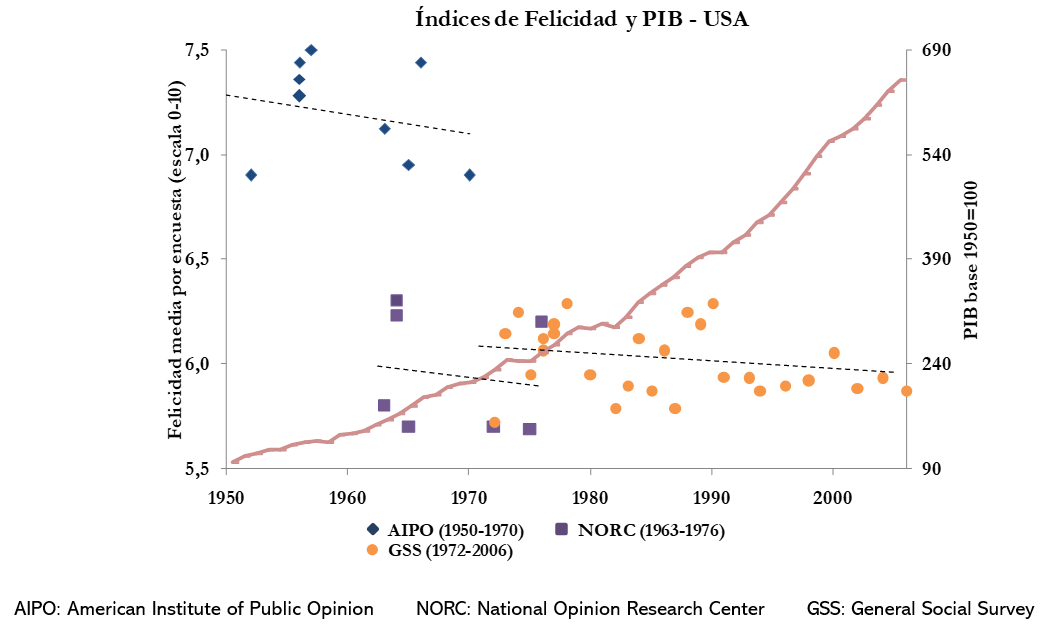
\includegraphics[scale=0.5]{Slides Principios de Economia/Figures/C17.2.png}
%\end{figure}
%\end{frame}

%\begin{frame}
%\frametitle{Idea más amplia de bienestar}
%\begin{itemize}
%    \item Enfoque de capacidades de Amartya Sen
%    \begin{itemize}
%        \item No es lo que una persona tiene, sino lo que ella es y puede hacer \\
%        - Capacidades para alcanzar su potencial como ser humano
%        \item ¿Disparidad entre los ingresos y las ventajas reales? \\
%        - Heterogeneidades personales, diversidad ambiental, diferencias en el clima social, distribución de recursos dentro de la familia, etc.
%    \end{itemize}
%    \item Índice de Desarrollo Humano (HDI) del PNUD
%    \begin{itemize}
%        \item Ingresos (PBI per cápita ajustado por PPP)
%        \item Longevidad (esperanza de vida al nacer)
%        \item Conocimiento (alfabetización y años de estudio0
%    \end{itemize}
%    \end{itemize}
%\end{frame}

\begin{frame}
\frametitle{PBI y desarrollo}
\begin{center}
    \href{https://ourworldindata.org/grapher/hdi-vs-gdp-per-capita} {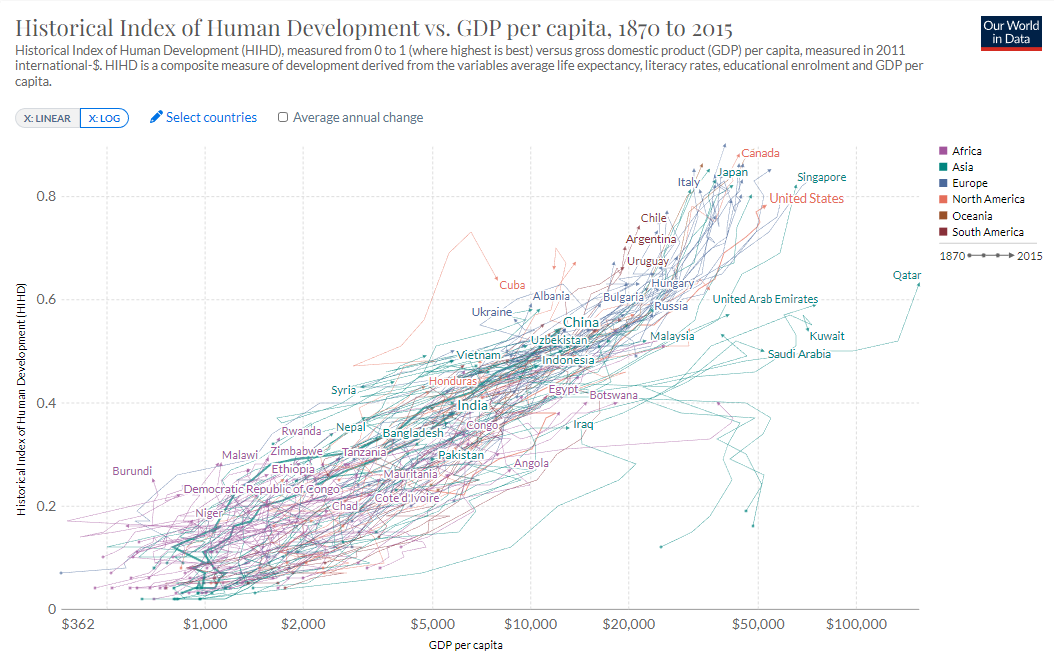
\includegraphics[scale=0.35]{Slides Principios de Economia/Tema_11.27_hdi_2.png}}
\end{center}
Fuente: Our World in Data
\end{frame}

\begin{frame}{Fuentes del crecimiento}
   \begin{equation*}
    Y = AF(K,L,H,RN),
\end{equation*} 
\begin{itemize}
    \item ¿El crecimiento viene de la acumulación de factores o de la tecnología?
    \item El hallazgo de Solow: la acumulación de factores no es suficiente para explicar el crecimiento.
\end{itemize}
\end{frame}

\begin{frame}{Un ejemplo de productividad}
    \begin{figure} [H]   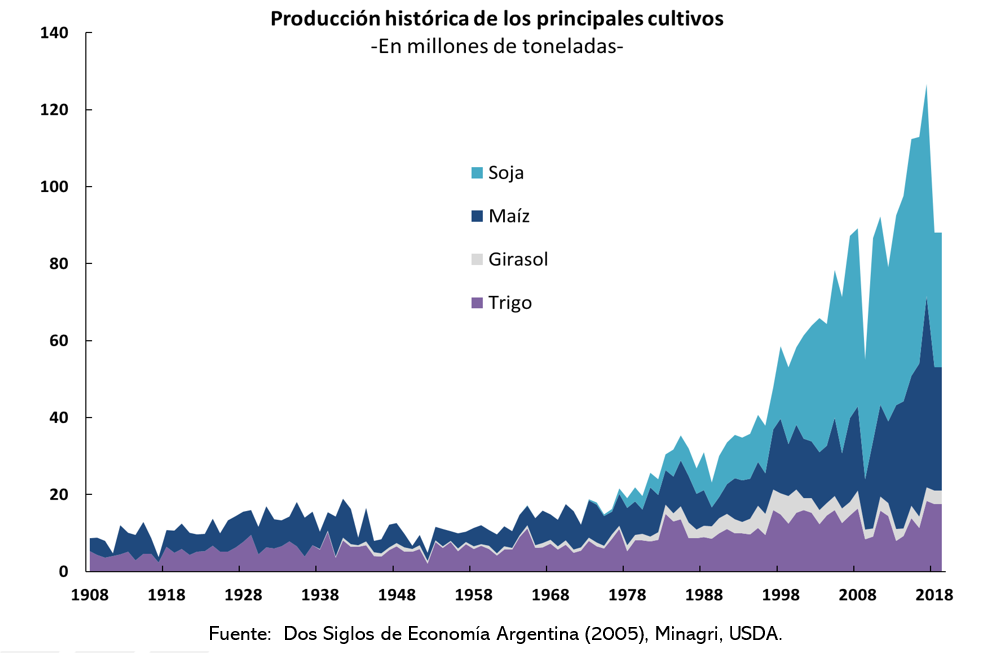
\includegraphics[scale=0.55]{Slides Principios de Economia/Figures/C17.3.png}
\label{fig:17.3}
\end{figure}
\end{frame}


\begin{frame}{La descomposición de crecimiento para Argentina}
    \begin{figure} [H]   
    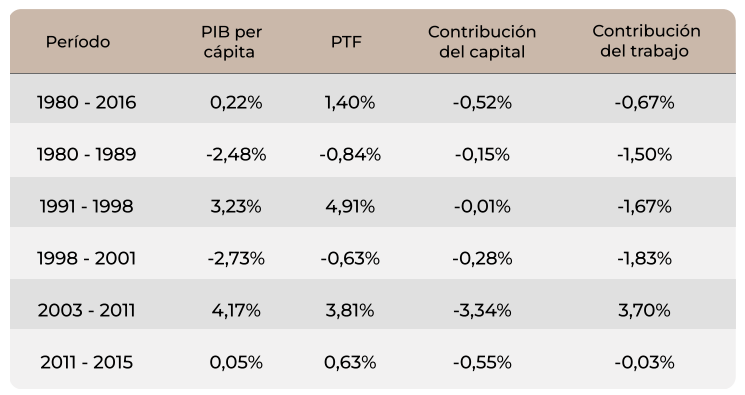
\includegraphics[scale=0.65]{Slides Principios de Economia/Figures/Magistral_20/C30.8.png}
\end{figure}
\end{frame}

\begin{frame}{Instituciones y Crecimiento}
    \begin{itemize}
        \item Dijimos que las instituciones son las reglas del juego en una sociedad
        \item \textbf{Instituciones económicas e instituciones políticas}
        \item Afectan de manera directa a los incentivos
        \item Establecen los incentivos para la innovación y el desarrollo tecnológico
        \item ¿Podemos evaluar de manera empírica el rol de las instituciones?
    \end{itemize}
    
    \begin{figure}[H]
        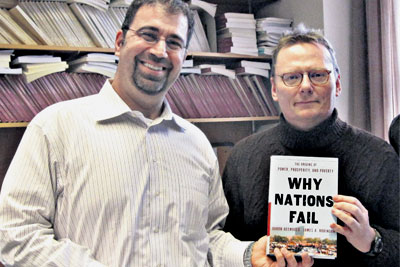
\includegraphics[scale=0.5]{../Figures/Acemoglurobinson.png}
    \end{figure}
\end{frame}

\begin{frame}{Instituciones}
    
\begin{figure}[H]
\begin{center}
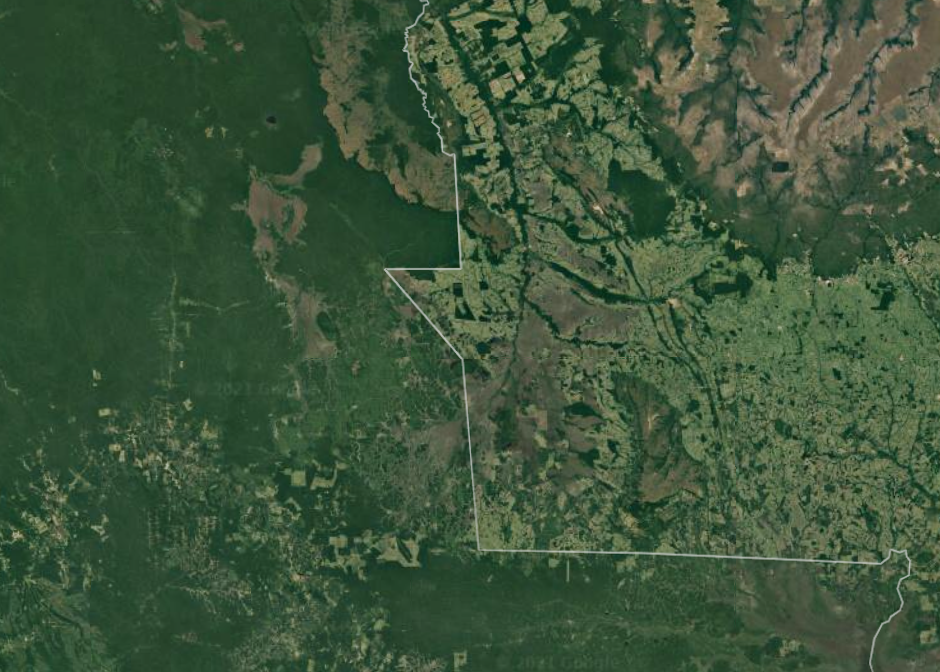
\includegraphics[width=0.8\textwidth]{Slides Principios de Economia/Figures/C26.2.png}
\end{center}
\caption{\textbf{Frontera entre Bolivia (izquierda) y Brazil}}
\label{fig:border_bol_bra}
\end{figure}
\end{frame}

\begin{frame}{Instituciones}
    \begin{figure}[H]
\begin{center}
\includegraphics[width=0.8\textwidth]{Slides Principios de Economia/Figures/C26.3.png}
\end{center}
\caption{\textbf{Península de Corea de noche}}
\label{fig:korea}
\end{figure}
\end{frame}

\begin{frame}{Desigualdad del Ingreso}
        \begin{itemize}
            \item Hay dos criterios para evaluar una asignación específica: 
            \begin{itemize}
                \item Eficiencia
                \item Equidad
            \end{itemize}
            \item ¿Existe un trade off entre eficiencia y equidad?
            \item Hay algunos factores importantes que determinan si una asignación es muy desigual:
            \begin{itemize}
                \item Diferencias en el poder de negociación
                \item Diferencias en sus dotaciones
                \item Instituciones
            \end{itemize}
            \item Para evaluar la desigualdad, los economistas a menudo usan unas medidas llamadas Coeficiente de Gini y Curva de Lorenz.
        \end{itemize}
\end{frame}

\begin{frame} 
\frametitle{La curva de Lorenz}
\begin{itemize}
\item Es una representación gráfica que muestra cómo se distribuye el ingreso entre la población de una economía o país. 
\item Para construirla, ordenamos en el eje horizontal a la población según su nivel de ingreso: desde las personas con menores ingresos a las personas con mayores ingresos.
\item En el eje vertical vamos reflejando el ingreso acumulado correspondiente al grupo que se está midiendo.
\item Para una sociedad con perfecta igualdad de ingresos, la curva de Lorenz sería una línea recta con una pendiente igual a uno.
\item Cuanto más alejada esté la curva de la línea de distribución equitativa (diagonal), más desigual será la sociedad.
\end{itemize}
\end{frame}

\begin{frame} 
\frametitle{Curva de Lorenz}
\begin{figure} [H]
\centering
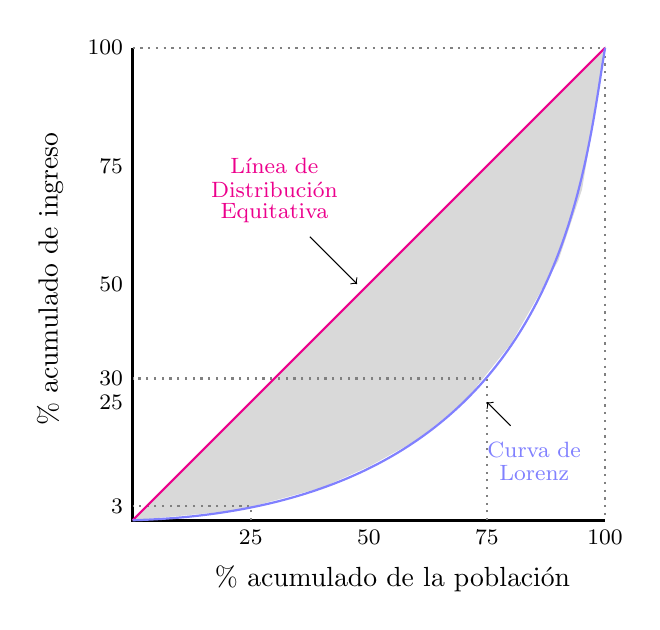
\begin{tikzpicture}[scale=0.6]
\draw[fill,gray!30] (0,0)--(10,10)--(9.5,7)--(9,5.5)--(8,3.75)--(7,2.5)--(6,1.7)--(5,1.15)--(4,0.7)--(2.15,0.2);
\draw[very thick,-] (0,10) node[above]{}--(0,0)--(10,0) node[right]{};
\draw[thick, dotted, gray] (0,10)--(10,10)--(10,0);
\draw[thick, dotted, gray] (2.5,0)--(2.5,0.3)--(0,0.3);
\draw[thick, dotted, gray] (7.5,0)--(7.5,3)--(0,3);
\draw[thick, magenta] (0,0)--(10,10);
\draw[thick, blue!50] (0,0)..controls (9,0.25) and (9.5,7)..(10,10);
\node at (-1.75, 5){\rotatebox{90}{ \% acumulado de ingreso}};
\node[] at (5.5,-1.25) { \% acumulado de la población};
\node[below] at (2.5,0){\footnotesize 25};
\node[below] at (5,0){\footnotesize 50};
\node[below] at (7.5,0){\footnotesize 75};
\node[below] at (10,0){\footnotesize 100};
\node[left] at (0,0.3){\footnotesize 3};
\node[left] at (0,2.5){\footnotesize 25};
\node[left] at (0,3){\footnotesize 30};
\node[left] at (0,5){\footnotesize 50};
\node[left] at (0,7.5){\footnotesize 75};
\node[left] at (0,10){\footnotesize 100};
\node[magenta] at (3,7.5) {\footnotesize Línea de };
\node[magenta] at (3,7) {\footnotesize Distribución};
\node[magenta] at (3,6.5) {\footnotesize Equitativa };
\draw[thin, ->] (3.75,6)--(4.75,5);
\node[blue!50] at (8.5,1.5) {\footnotesize Curva de };
\node[blue!50] at (8.5,1) {\footnotesize Lorenz };
\draw[thin, ->] (8,2)--(7.5,2.5);
\end{tikzpicture}
\end{figure} 
\end{frame}

\begin{frame} 
\frametitle{El coeficiente de Gini y la curva de Lorenz}
\begin{itemize}
\item Para comparar la desigualdad a lo largo del tiempo o entre dos países utilizamos el Índice de Gini. \vspace{1mm}
\item El índice se puede aproximar como el área entre la diagonal de perfecta igualdad y la curva de Lorenz (A) dividida sobre la superficie total del área del triángulo inferior derecho (A+B): \\ \vspace{1mm}
\begin{center}
   $G=\frac{A}{A+B}$ 
\end{center} \vspace{1mm}
\item Si no hay desigualdad de ingresos, el coeficiente de Gini es 0. Esto se debe a que la curva de Lorenz sería exactamente la línea de la igualdad perfecta, por lo que no habría área entre los dos

\end{itemize}
\end{frame}

\begin{frame} 
\frametitle{El coeficiente de Gini y la curva de Lorenz}
\begin{figure} [H]
\centering
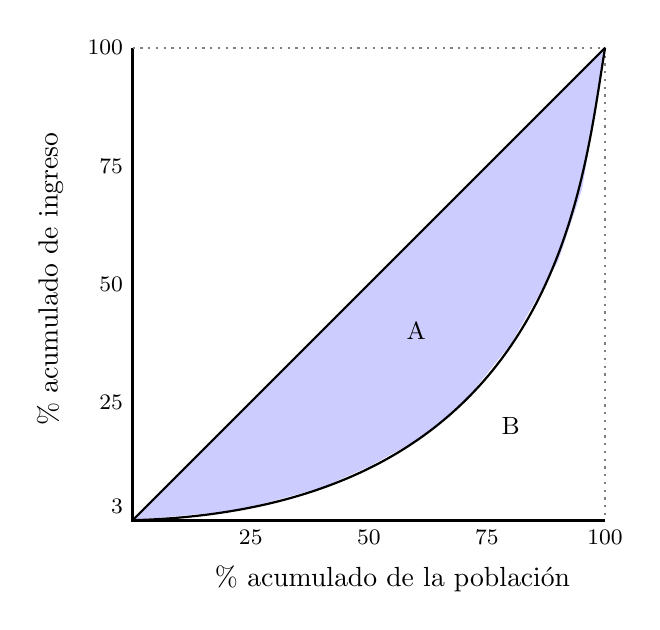
\begin{tikzpicture}[scale=0.6]
\draw[fill,blue!20] (0,0)--(10,10)--(9.5,7)--(9,5.5)--(8,3.75)--(7,2.5)--(6,1.7)--(5,1.15)--(4,0.7)--(2.15,0.2);
\draw[very thick,-] (0,10) node[above]{}--(0,0)--(10,0) node[right]{};
\draw[thick, dotted, gray] (0,10)--(10,10)--(10,0);
\draw[thick] (0,0)--(10,10);
\draw[thick] (0,0)..controls (9,0.25) and (9.5,7)..(10,10);
\node at (-1.75, 5){\rotatebox{90}{ \% acumulado de ingreso}};
\node[] at (5.5,-1.25) { \% acumulado de la población};
\node[below] at (2.5,0){\footnotesize 25};
\node[below] at (5,0){\footnotesize 50};
\node[below] at (7.5,0){\footnotesize 75};
\node[below] at (10,0){\footnotesize 100};
\node[left] at (0,0.3){\footnotesize 3};
\node[left] at (0,2.5){\footnotesize 25};
\node[left] at (0,5){\footnotesize 50};
\node[left] at (0,7.5){\footnotesize 75};
\node[left] at (0,10){\footnotesize 100};

\node[] at (6,4) {\small A };
\node[] at (8,2) {\small B };

\end{tikzpicture}
\end{figure} 
\end{frame}

\begin{frame} 
\frametitle{Un ejemplo aplicado}
    \begin{center}    
    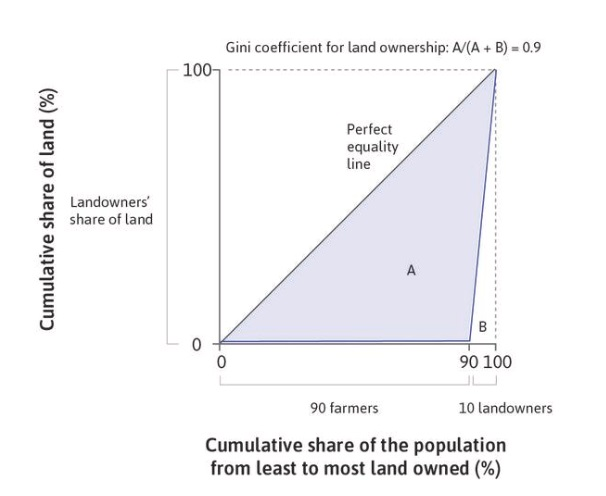
\includegraphics[scale=0.55]{../Figures/Tema_04.18_lorenz3.jpg}
    \end{center}
\end{frame}

\begin{frame} 
\frametitle{Un ejemplo aplicado}
    \begin{center}    
    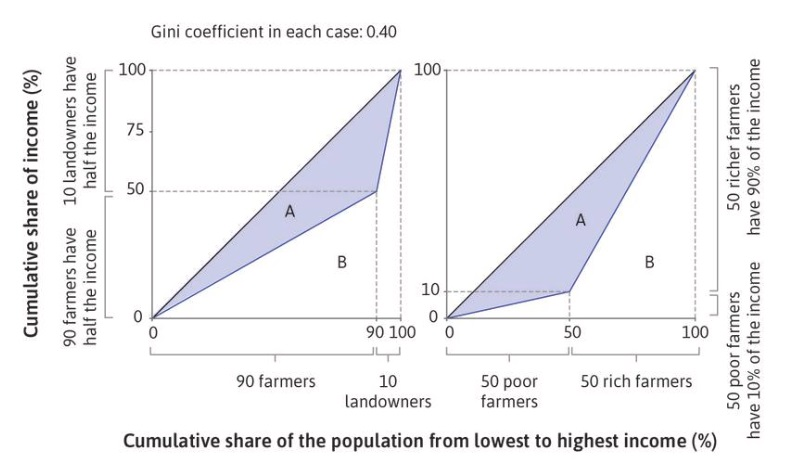
\includegraphics[scale=0.55]{../Figures/Tema_04.20_variedaddesigual.jpg}
    \end{center}
\end{frame}

\begin{frame} 
\frametitle{Diferentes variedad de desigualdad}
\begin{itemize}
\item En la figura anterior hay dos sociedades con el mismo coeficiente de Gini.
\item El área $\frac{A}{A + B}$ es la misma en cada curva de Lorenz, pero la distribución del ingreso está lejos de ser idéntica.
\item En la sociedad de la izquierda, la mitad del ingreso total se divide entre 90 agricultores mientras que 10 terratenientes obtienen la mitad restante. 
\item En la sociedad que se muestra a la derecha, 50 agricultores pobres obtienen una décima parte de los ingresos para dividirse entre ellos y 50 agricultores más ricos dividen el 90\% restante.
\end{itemize}
\end{frame}

\begin{frame} 
\frametitle{Diferentes variedad de desigualdad}
\begin{itemize}
\item ¡No todas las desigualdades son iguales!
\item No es lo mismo que una sociedad sea altamente desigual porque hay un pequeño número de personas excepcionalmente ricas y todos los demás están en una situación de buena posición económica o que sea desigual porque hay un pequeño número de personas muy pobres, y todos los demás están en mejores condiciones
\item Estas dos sociedades podrían tener el mismo coeficiente de Gini, pero pensaríamos que son bastante diferentes en la naturaleza de la desigualdad que experimentan
\end{itemize}
\end{frame}


\end{document}